% Chapter 4: Methodology
\chapter{Methodology}

This chapter presents the comprehensive methodology used in the development of the Timetable Buddy system. It includes various modeling diagrams, project management artifacts, and quality assurance documentation that guided the systematic development approach for creating a robust lecture scheduling solution.

\section{Data Flow Diagrams (DFD)}

Data Flow Diagrams represent the flow of data through the system at different levels of abstraction, showing how information moves between processes, data stores, and external entities in the Timetable Buddy system.

\subsection{DFD Level 0 (Context Diagram)}

The Context Diagram provides a high-level view of the entire Timetable Buddy system, showing its interaction with external entities including Students, Faculty, and Administrators.

\begin{figure}[ht]
    \centering
    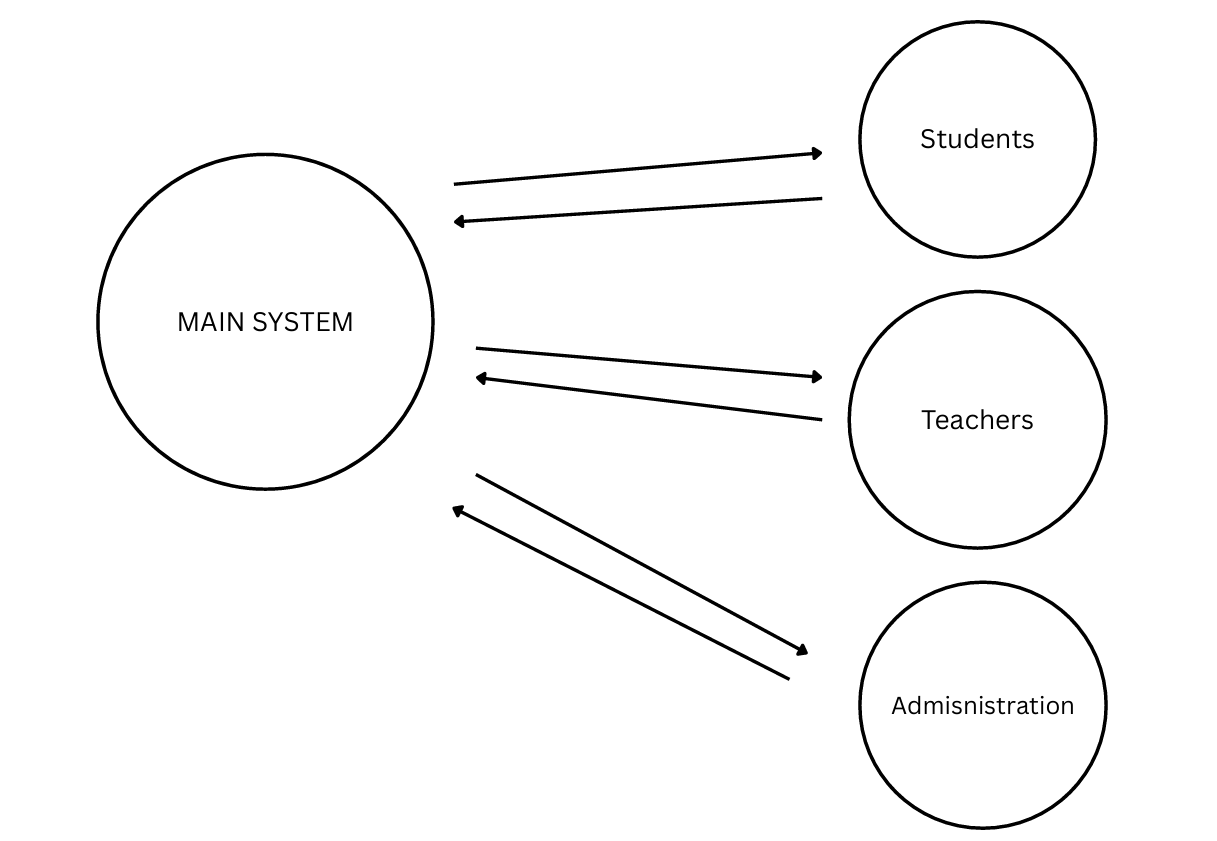
\includegraphics[width=0.85\textwidth]{images/DFD Level 0.png}
    \caption{DFD Level 0 - Context Diagram showing system boundaries and external entities}
    \label{fig:dfd0}
\end{figure}

The context diagram illustrates:
\begin{itemize}[leftmargin=*]
    \item \textbf{External Entities:} Students, Faculty, Administrators
    \item \textbf{Main System:} Timetable Buddy System (central process)
    \item \textbf{Data Flows:} Authentication requests, enrollment data, lecture schedules, timetable information
    \item \textbf{System Boundary:} Clear delineation between internal processes and external interactions
\end{itemize}

\subsection{DFD Level 1 (High-Level Processes)}

Level 1 DFD decomposes the main system into major processes, showing the primary functional components and their interactions with data stores and external entities.

\begin{figure}[ht]
    \centering
    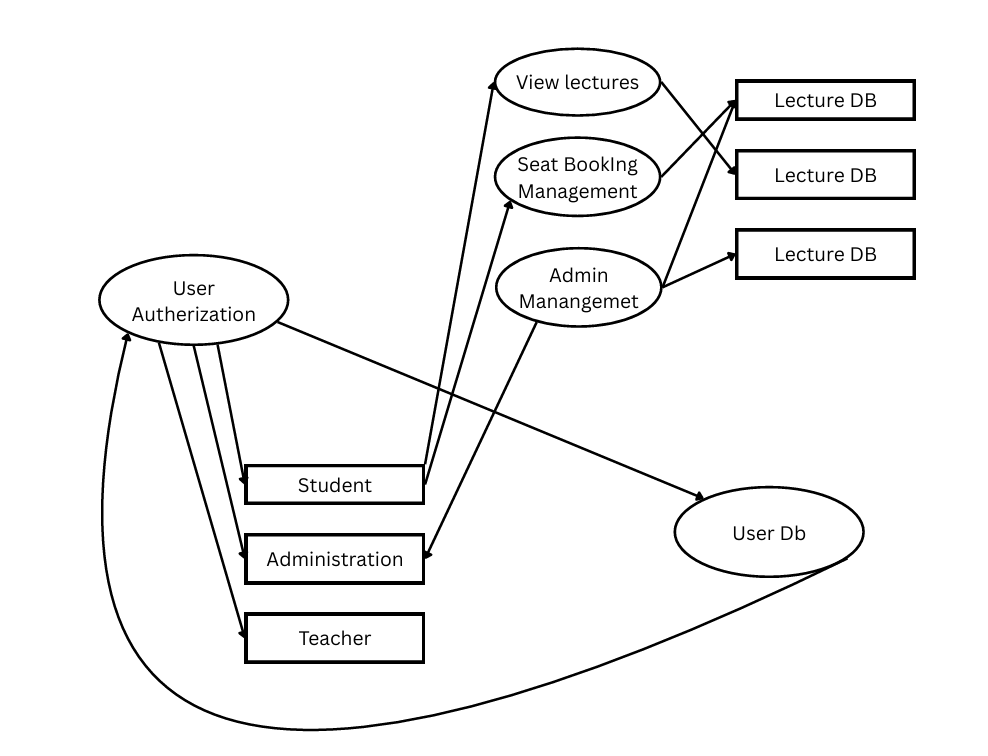
\includegraphics[width=0.95\textwidth]{images/DFD Level 1.png}
    \caption{DFD Level 1 - Major system processes and data stores}
    \label{fig:dfd1}
\end{figure}

Key processes shown in Level 1 include:
\begin{itemize}[leftmargin=*]
    \item \textbf{Process 1:} User Authentication and Authorization
    \item \textbf{Process 2:} Lecture Slot Management
    \item \textbf{Process 3:} Enrollment Processing
    \item \textbf{Process 4:} Timetable Generation and Display
    \item \textbf{Process 5:} Dashboard and Analytics
    \item \textbf{Data Stores:} User Database, Lecture Slots, Enrollments, Schedules
\end{itemize}

\subsection{DFD Level 2 (Detailed Processes)}

Level 2 DFD provides detailed decomposition of complex processes from Level 1, showing sub-processes and their detailed interactions within the enrollment management system.

\begin{figure}[h]
    \centering
    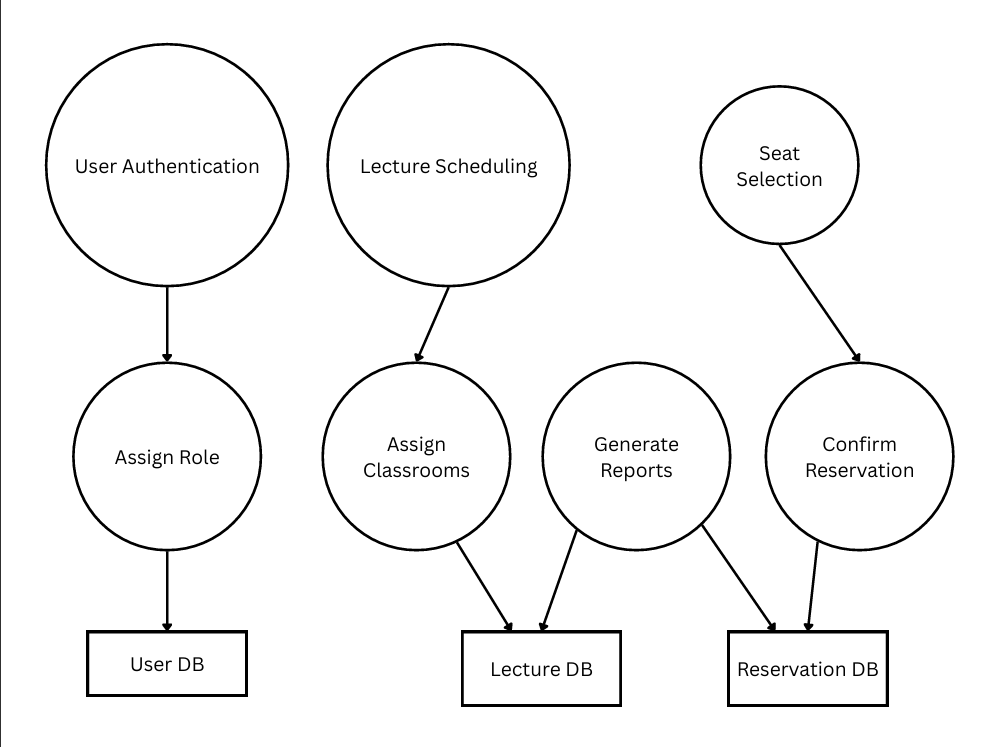
\includegraphics[width=0.95\textwidth]{images/DFD Level 2.png}
    \caption{DFD Level 2 - Detailed process decomposition}
    \label{fig:dfd2}
\end{figure}

The Level 2 diagram details:
\begin{itemize}[leftmargin=*]
    \item Enrollment workflow with waitlist management
    \item Conflict detection mechanisms
    \item Capacity validation processes
    \item Notification generation
\end{itemize}

\section{Use Case Diagram}

The Use Case Diagram illustrates the functional requirements from the user's perspective, showing the interactions between different actors and the system use cases.

\begin{figure}[h]
    \centering
    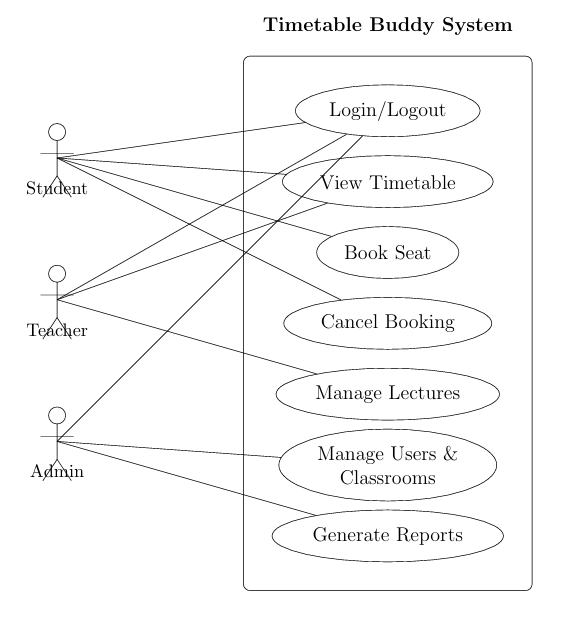
\includegraphics[width=0.85\textwidth]{images/Usecase diagram.png}
    \caption{Use Case Diagram showing actor interactions and system use cases}
    \label{fig:usecase}
\end{figure}

\textbf{Actors:}
\begin{itemize}[leftmargin=*]
    \item \textbf{Student:} Can view timetables, enroll in courses, manage profile, view enrollment status
    \item \textbf{Faculty:} Can manage lecture slots, view enrolled students, update course details
    \item \textbf{Administrator:} Can manage users, courses, lecture slots, generate reports, configure system settings
\end{itemize}

\textbf{Key Use Cases:}
\begin{itemize}[leftmargin=*]
    \item User Authentication (Login/Logout)
    \item Manage Lecture Slots
    \item Enroll in Courses
    \item View Timetable
    \item Manage Enrollments
    \item Generate Reports
    \item User Management
\end{itemize}

\section{Sequence Diagram}

Sequence Diagrams show the interaction between objects over time, illustrating the message flow and order of operations for specific scenarios.

\begin{figure}[h]
    \centering
    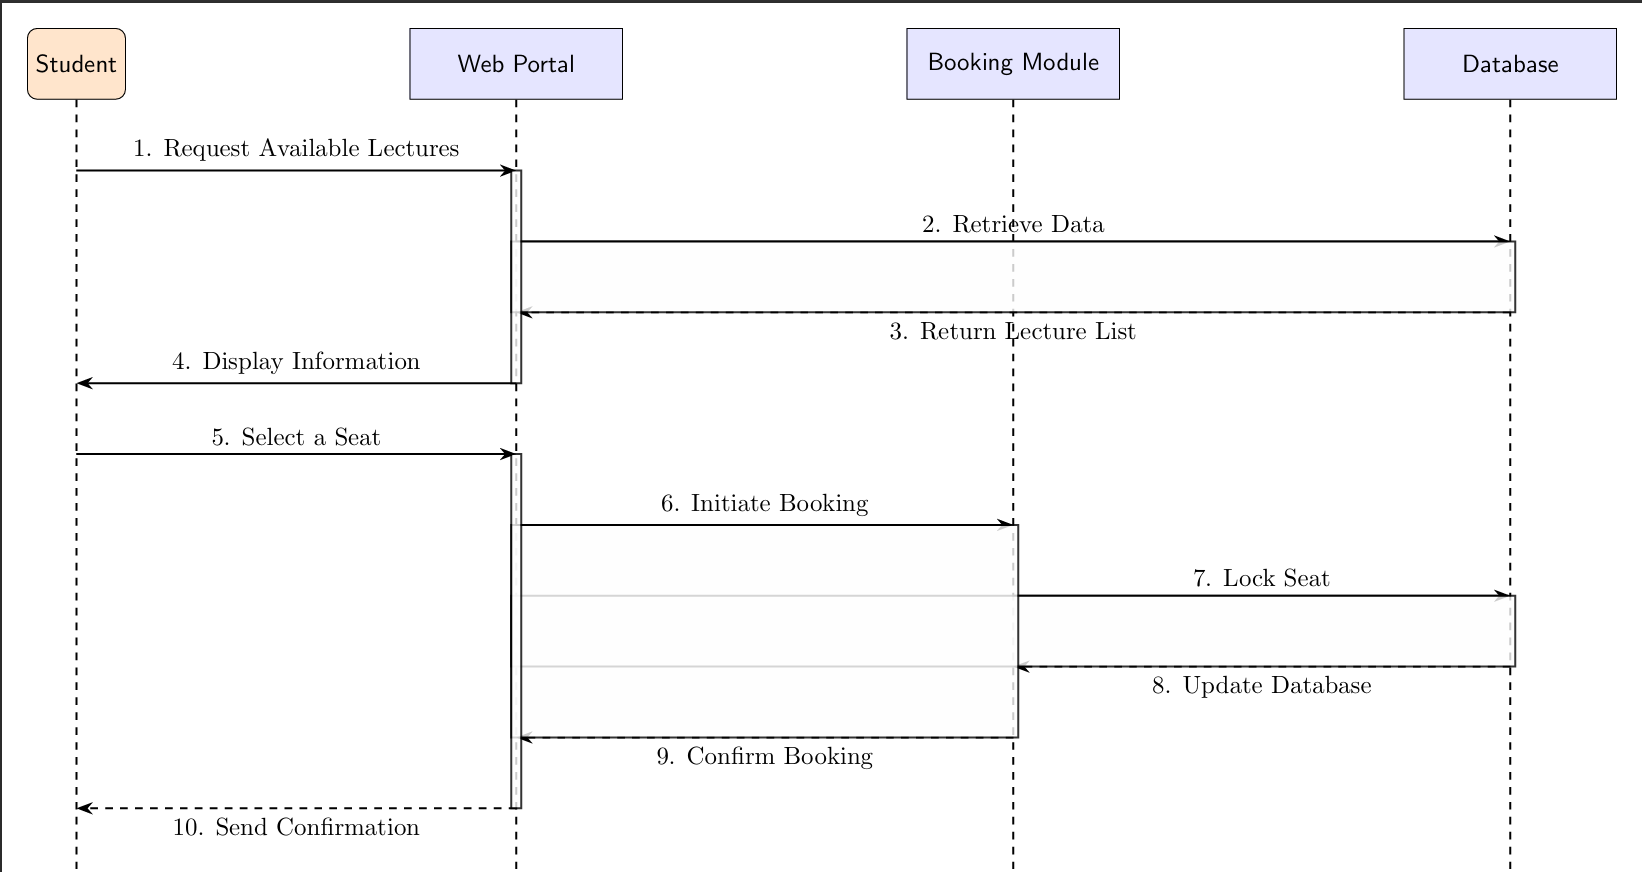
\includegraphics[width=0.95\textwidth]{images/Sequence Diagram.png}
    \caption{Sequence Diagram showing object interactions for enrollment process}
    \label{fig:sequence}
\end{figure}

The sequence diagram depicts:
\begin{itemize}[leftmargin=*]
    \item User authentication flow
    \item Enrollment request processing
    \item Conflict detection validation
    \item Capacity checking
    \item Database operations
    \item Response generation
\end{itemize}

\section{Activity Diagram}

Activity Diagrams model the workflow and business logic, showing the sequence of activities and decision points in system processes.

\begin{figure}[h]
    \centering
    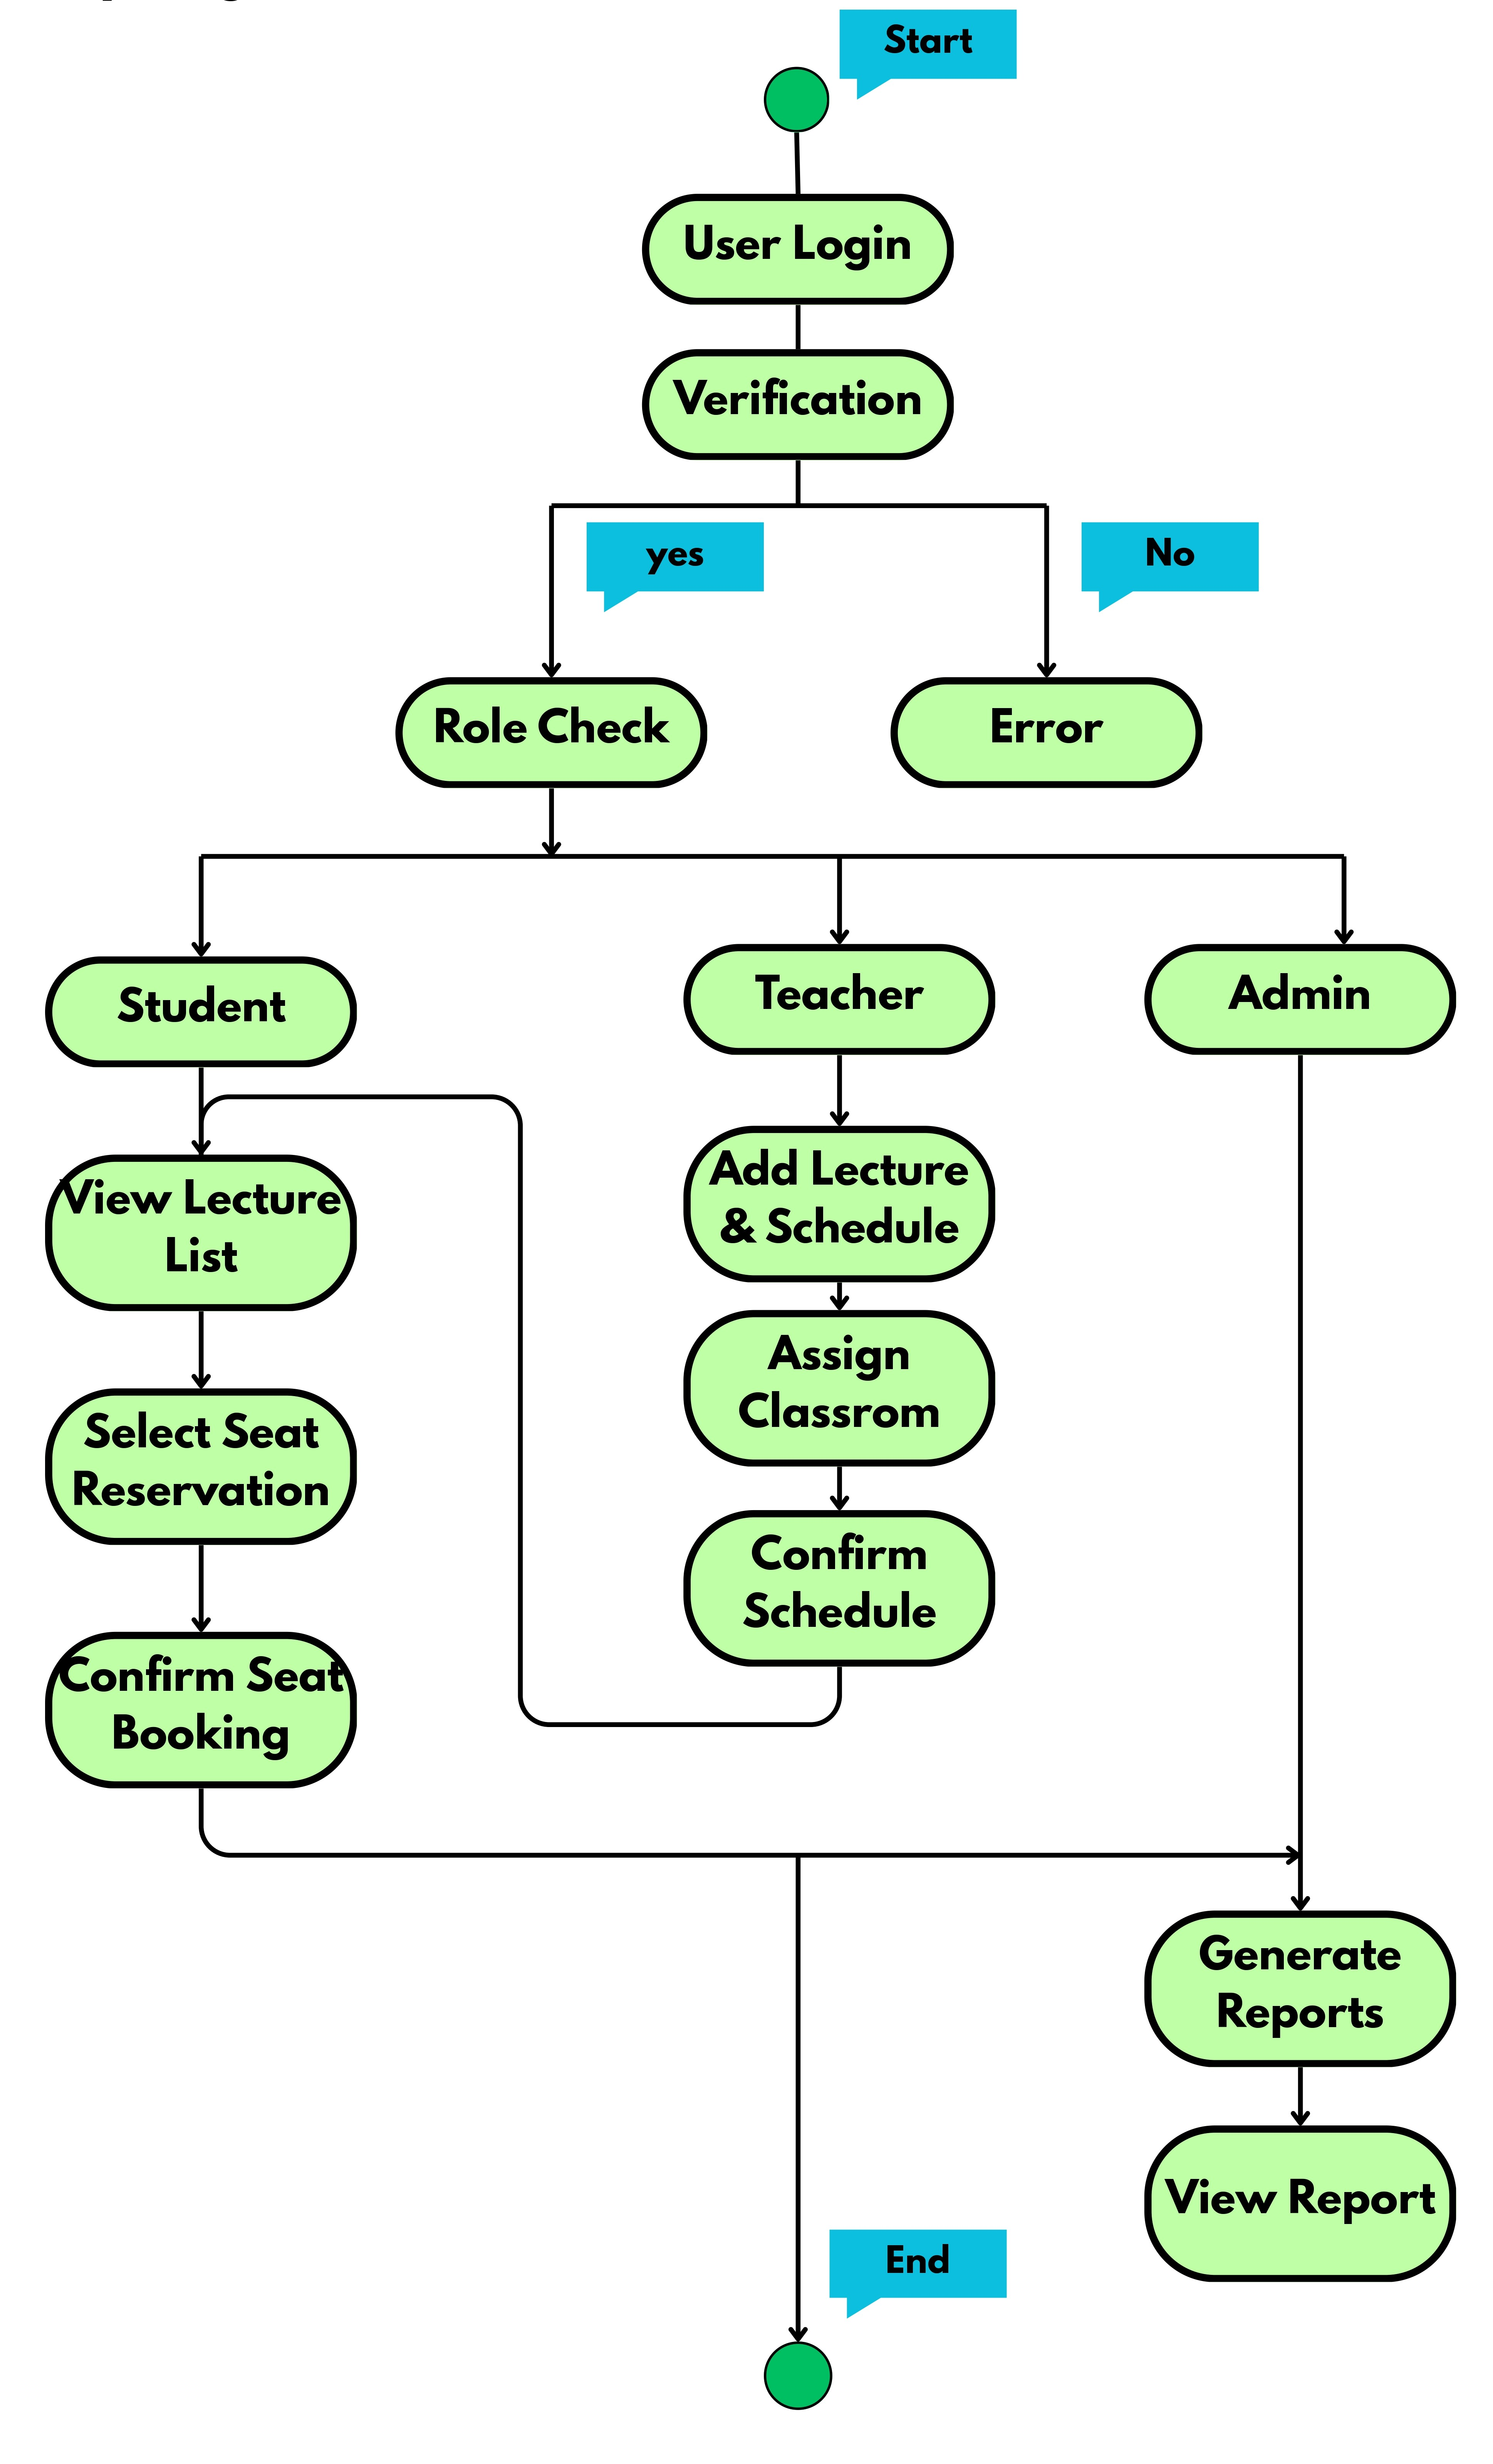
\includegraphics[width=0.75\textwidth]{images/Activity Diagram.jpg}
    \caption{Activity Diagram illustrating enrollment workflow and decision logic}
    \label{fig:activity}
\end{figure}

The activity diagram illustrates:
\begin{itemize}[leftmargin=*]
    \item Enrollment process workflow
    \item Decision points for capacity checks
    \item Conflict detection logic
    \item Waitlist management
    \item Success and failure paths
\end{itemize}

\section{Deployment Diagram}

The Deployment Diagram shows the physical architecture of the system, illustrating how software components are deployed on hardware nodes.

\begin{figure}[h]
    \centering
    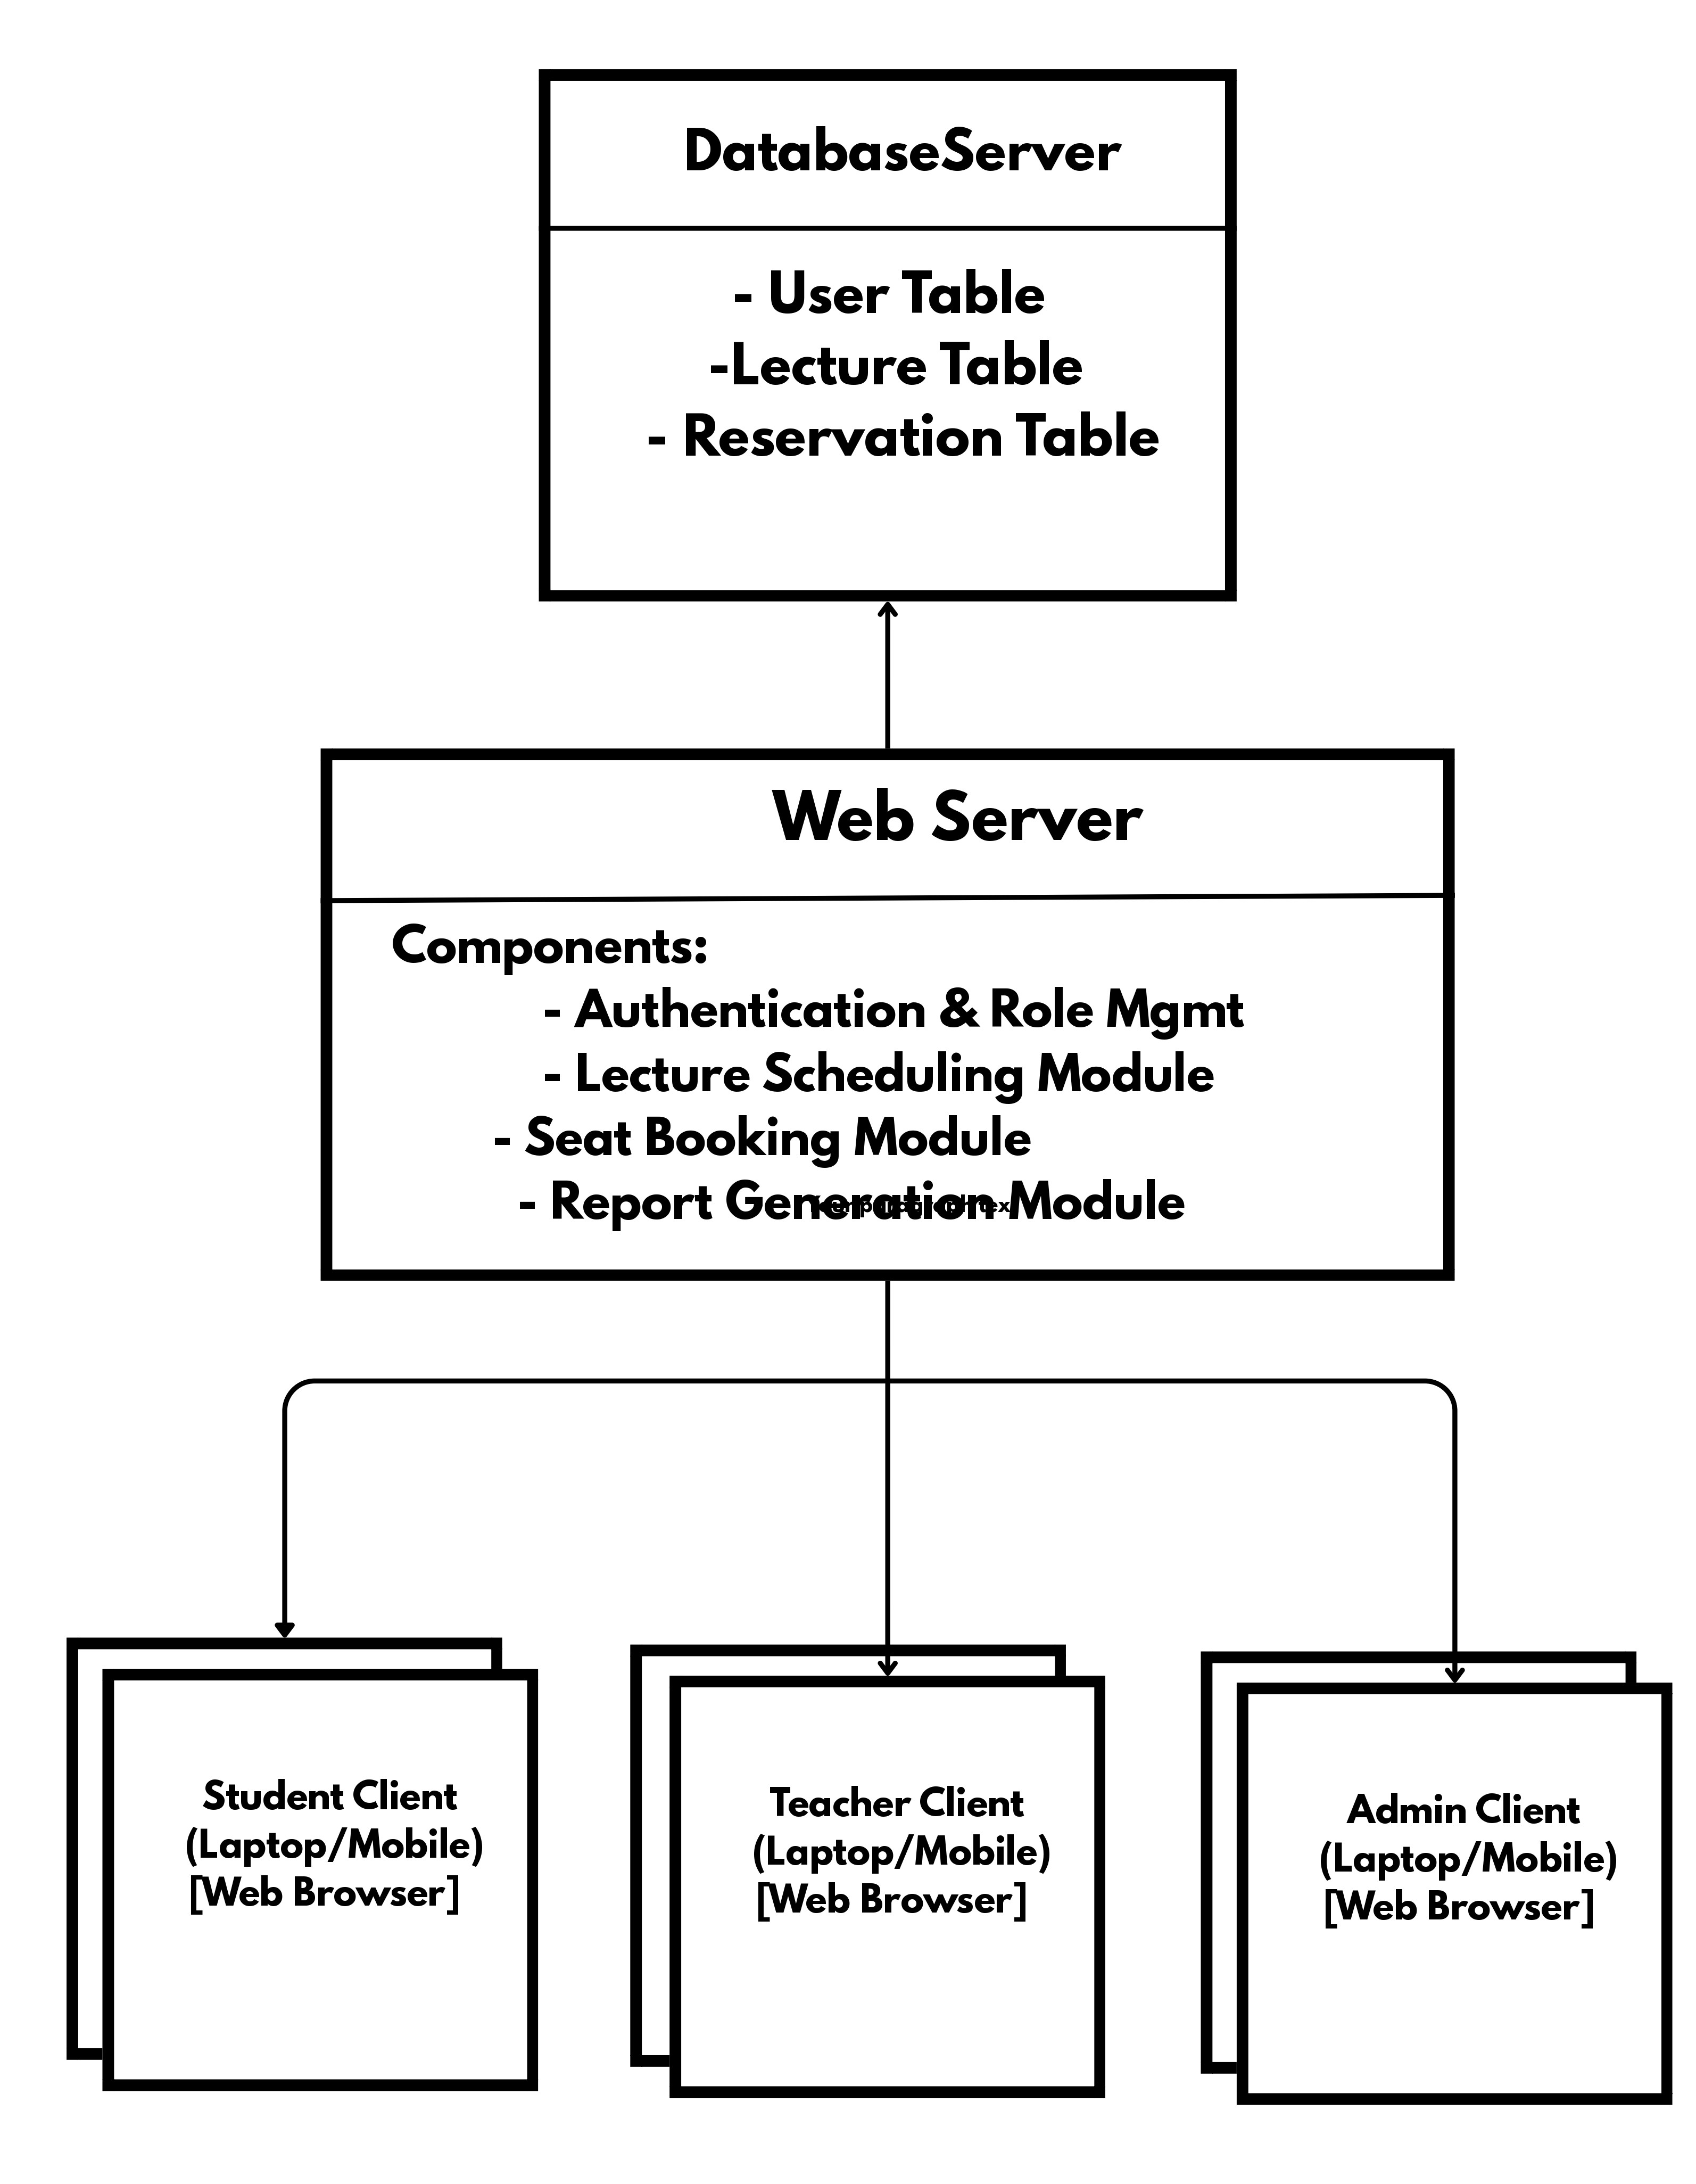
\includegraphics[width=0.85\textwidth]{images/Deployment Diagram.jpg}
    \caption{Deployment Diagram showing system architecture and component deployment}
    \label{fig:deployment}
\end{figure}

\textbf{System Components:}
\begin{itemize}[leftmargin=*]
    \item \textbf{Client Layer:} Web browsers on user devices
    \item \textbf{Application Layer:} React frontend, Node.js backend
    \item \textbf{Database Layer:} MongoDB database server
    \item \textbf{Deployment:} Docker containers for containerized deployment
\end{itemize}

\textbf{Communication Protocols:}
\begin{itemize}[leftmargin=*]
    \item HTTPS for client-server communication
    \item REST API for frontend-backend interaction
    \item MongoDB protocol for database connections
\end{itemize}

\section{Work Breakdown Structure (WBS)}

The Work Breakdown Structure decomposes the project into manageable components, showing the hierarchical breakdown of deliverables and tasks.

\begin{figure}[h]
    \centering
    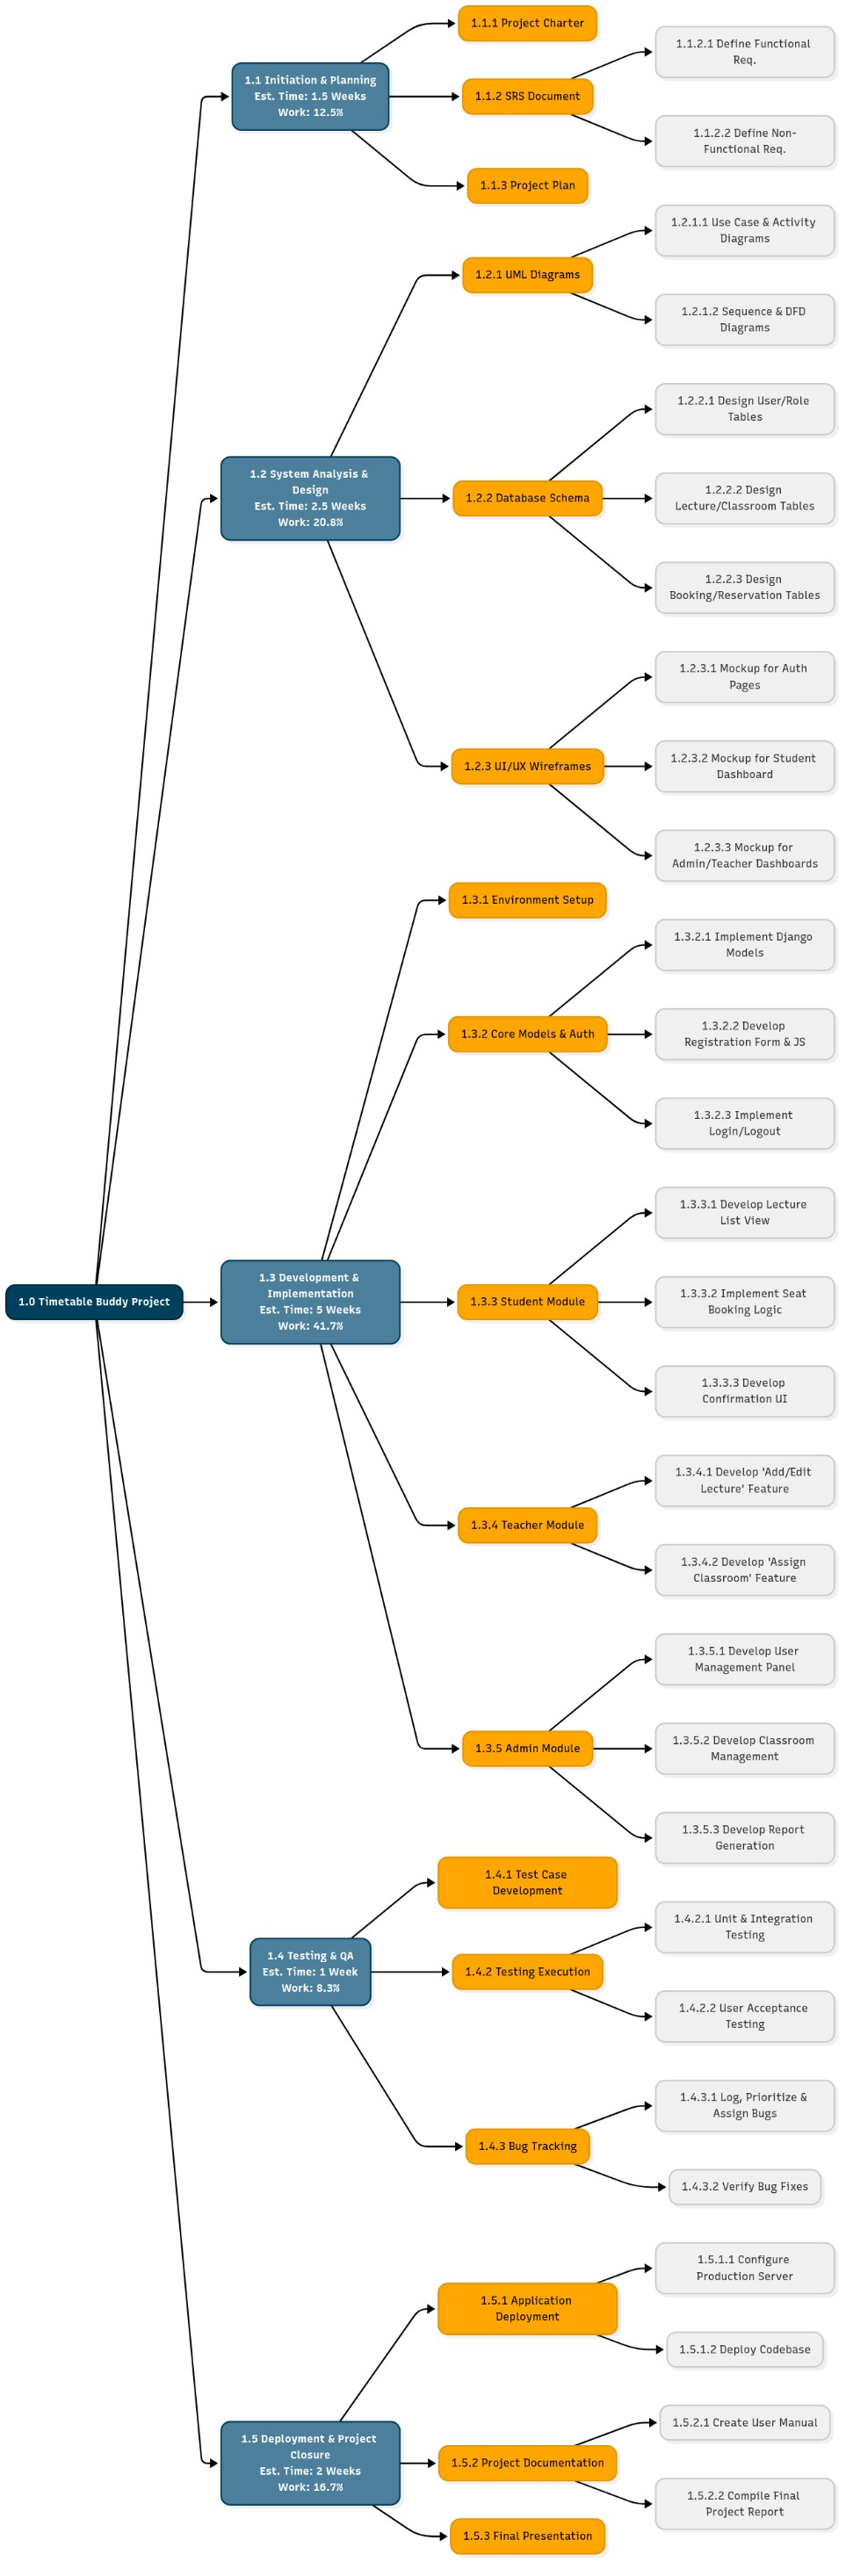
\includegraphics[width=0.95\textwidth]{images/WBS.jpg}
    \caption{Work Breakdown Structure showing project task hierarchy}
    \label{fig:wbs}
\end{figure}

\textbf{Major Work Packages:}
\begin{enumerate}[leftmargin=*]
    \item \textbf{Project Planning:} Requirements gathering, feasibility analysis, project plan
    \item \textbf{Design:} System architecture, database design, UI/UX design, API design
    \item \textbf{Development:} Frontend development, backend development, database implementation
    \item \textbf{Testing:} Unit testing, integration testing, system testing, user acceptance testing
    \item \textbf{Deployment:} Environment setup, deployment, documentation
    \item \textbf{Project Management:} Risk management, quality assurance, documentation
\end{enumerate}

\section{Gantt Chart}

The Gantt Chart provides a timeline view of project activities, showing task dependencies, durations, and milestones.

\begin{figure}[h]
    \centering
    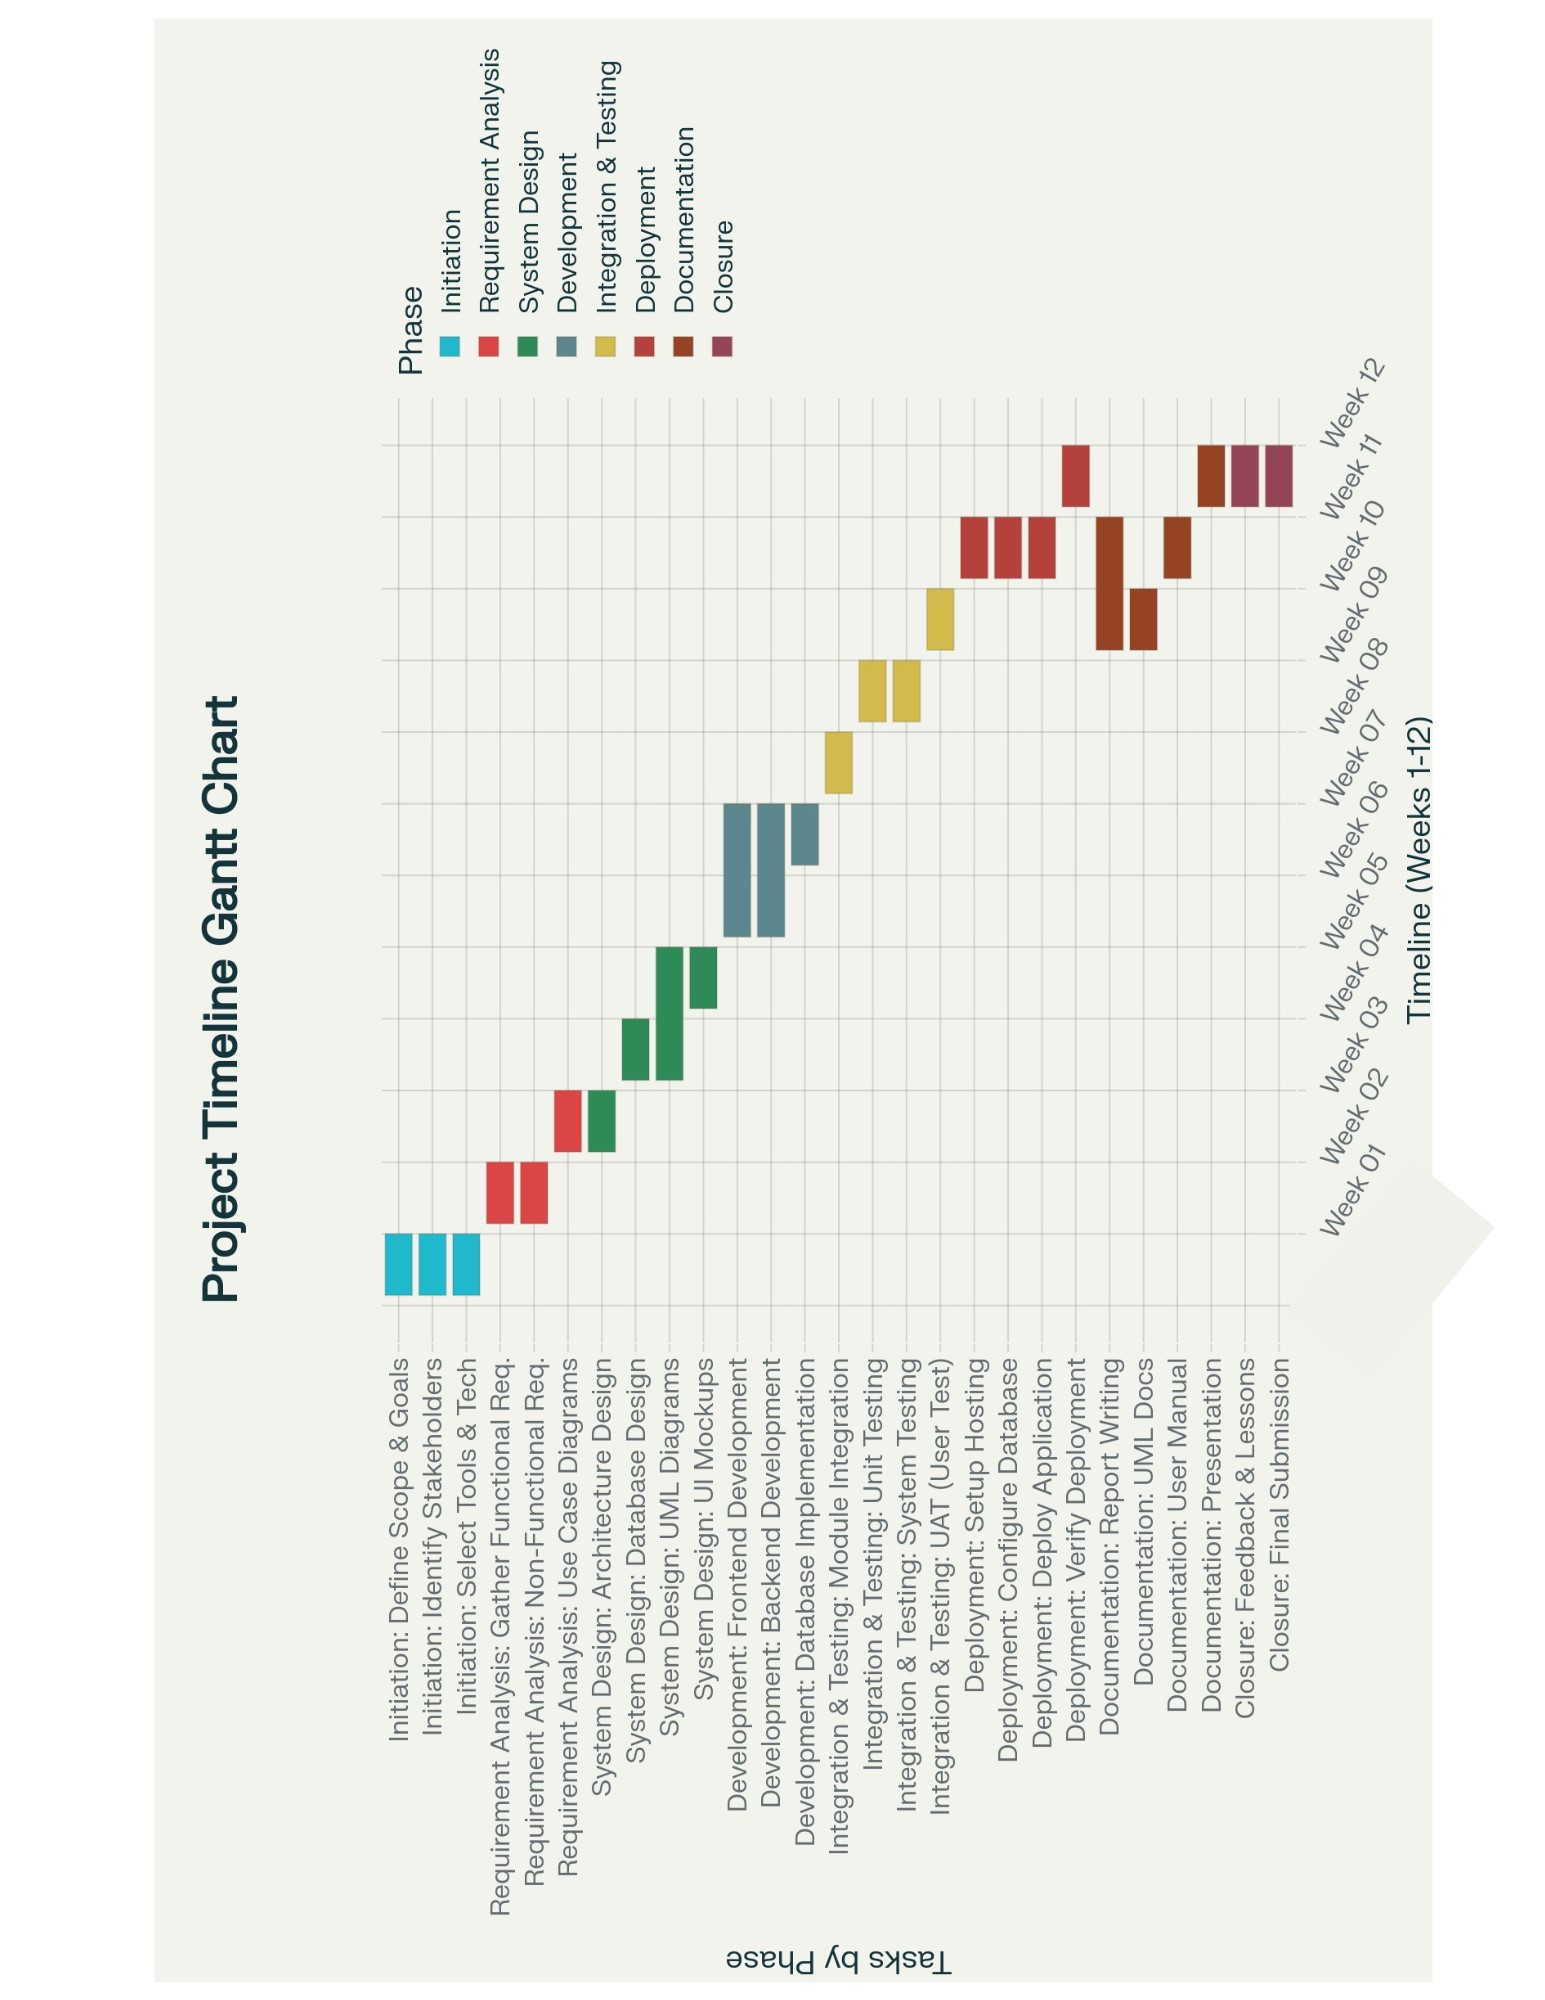
\includegraphics[width=0.95\textwidth]{images/Gantt Chart.jpg}
    \caption{Gantt Chart showing project timeline and task scheduling}
    \label{fig:gantt}
\end{figure}

\textbf{Project Phases and Timeline:}
\begin{itemize}[leftmargin=*]
    \item \textbf{Phase 1 - Planning:} Requirements analysis, feasibility study, project planning
    \item \textbf{Phase 2 - Design:} System design, database design, UI mockups
    \item \textbf{Phase 3 - Development:} Frontend and backend implementation
    \item \textbf{Phase 4 - Testing:} Comprehensive testing across all modules
    \item \textbf{Phase 5 - Deployment:} Production deployment and user training
\end{itemize}

\section{RMMM Plan (Risk Management, Monitoring, and Mitigation)}

The RMMM Plan provides a comprehensive framework for identifying, assessing, monitoring, and mitigating project risks throughout the development lifecycle.

\subsection{Risk Identification and Assessment}

Risks have been identified across technical, operational, and external categories. Each risk is assessed for probability and impact, with detailed mitigation strategies. This document includes only risks with a probability of 15\% or less, as higher probability risks are managed through other project management processes.

\textbf{Risk Assessment Criteria:}
\begin{itemize}[leftmargin=*]
    \item \textbf{Probability Levels:} Only risks with $\leq$15\% probability are included
    \item \textbf{Impact Levels:} Critical, High, Medium, Low
\end{itemize}

\textbf{Risk Categories:}
\begin{itemize}[leftmargin=*]
    \item \textbf{Technical Risks:} Technology failures, integration issues, performance problems, security vulnerabilities
    \item \textbf{Operational Risks:} Resource availability, skill gaps, schedule delays
    \item \textbf{External Risks:} Third-party dependencies, requirement changes, infrastructure issues
\end{itemize}

\subsection{Detailed Risk Assessment}

\subsubsection{Risk \#1: R-TTB-005}

\begin{table}[h]
\small
\begin{tabular}{|p{3cm}|p{3cm}|p{3cm}|p{3cm}|}
\hline
\textbf{Risk ID} & R-TTB-005 & \textbf{Type} & Technical \\
\hline
\textbf{Probability} & 10\% & \textbf{Impact} & Critical \\
\hline
\end{tabular}
\end{table}

\textbf{Risk Description:} Critical security vulnerability discovered in production system allowing unauthorized data access.

\textbf{Mitigation Plan:}
\begin{enumerate}[leftmargin=*]
    \item Conduct regular security audits and penetration testing
    \item Implement security scanning in CI/CD pipeline
    \item Follow OWASP guidelines for secure development
\end{enumerate}

\textbf{Monitoring Plan:} Run automated security scans weekly. Monitor security patch releases for dependencies.

\textbf{Management Plan:} Deploy emergency patch within 4 hours. Notify affected users. Conduct incident post-mortem.

\subsubsection{Risk \#2: R-TTB-008}

\begin{table}[h]
\small
\begin{tabular}{|p{3cm}|p{3cm}|p{3cm}|p{3cm}|}
\hline
\textbf{Risk ID} & R-TTB-008 & \textbf{Type} & Technical \\
\hline
\textbf{Probability} & 15\% & \textbf{Impact} & High \\
\hline
\end{tabular}
\end{table}

\textbf{Risk Description:} Cloud service provider experiences prolonged outage affecting application availability.

\textbf{Mitigation Plan:}
\begin{enumerate}[leftmargin=*]
    \item Implement multi-region deployment
    \item Design for high availability
    \item Have disaster recovery plan in place
\end{enumerate}

\textbf{Monitoring Plan:} Subscribe to cloud provider status updates. Monitor service health across regions.

\textbf{Management Plan:} Failover to backup region. Communicate status to users. Document incident for review.

\subsubsection{Risk \#3: R-TTB-015}

\begin{table}[h]
\small
\begin{tabular}{|p{3cm}|p{3cm}|p{3cm}|p{3cm}|}
\hline
\textbf{Risk ID} & R-TTB-015 & \textbf{Type} & External \\
\hline
\textbf{Probability} & 15\% & \textbf{Impact} & High \\
\hline
\end{tabular}
\end{table}

\textbf{Risk Description:} Vendor lock-in prevents migration to alternative solutions, increasing long-term costs.

\textbf{Mitigation Plan:}
\begin{enumerate}[leftmargin=*]
    \item Use open standards where possible
    \item Design abstraction layers for vendor services
    \item Evaluate vendor independence regularly
\end{enumerate}

\textbf{Monitoring Plan:} Review vendor contracts annually. Assess switching costs and alternatives.

\textbf{Management Plan:} Plan phased migration to alternative vendor. Negotiate better terms with current vendor. Implement vendor-agnostic architecture.

\subsubsection{Risk \#4: R-TTB-018}

\begin{table}[h]
\small
\begin{tabular}{|p{3cm}|p{3cm}|p{3cm}|p{3cm}|}
\hline
\textbf{Risk ID} & R-TTB-018 & \textbf{Type} & External \\
\hline
\textbf{Probability} & 12\% & \textbf{Impact} & Critical \\
\hline
\end{tabular}
\end{table}

\textbf{Risk Description:} Competitor launches similar product first, reducing market opportunity.

\textbf{Mitigation Plan:}
\begin{enumerate}[leftmargin=*]
    \item Conduct competitive analysis regularly
    \item Focus on unique value propositions
    \item Plan for rapid iteration and deployment
\end{enumerate}

\textbf{Monitoring Plan:} Monitor competitor activities and product launches. Track market trends and customer feedback.

\textbf{Management Plan:} Accelerate development of differentiating features. Adjust marketing strategy. Consider strategic partnerships.

\subsubsection{Risk \#5: R-TTB-024}

\begin{table}[h]
\small
\begin{tabular}{|p{3cm}|p{3cm}|p{3cm}|p{3cm}|}
\hline
\textbf{Risk ID} & R-TTB-024 & \textbf{Type} & Operational \\
\hline
\textbf{Probability} & 15\% & \textbf{Impact} & High \\
\hline
\end{tabular}
\end{table}

\textbf{Risk Description:} Inadequate disaster recovery procedures lead to extended downtime after incident.

\textbf{Mitigation Plan:}
\begin{enumerate}[leftmargin=*]
    \item Document and test DR procedures quarterly
    \item Automate recovery processes
    \item Maintain offsite backups
\end{enumerate}

\textbf{Monitoring Plan:} Test disaster recovery plan every 6 months. Track RTO and RPO metrics.

\textbf{Management Plan:} Execute disaster recovery plan. Communicate with stakeholders. Document incident for improvement.

\subsection{Risk Management Process}

\textbf{1. Risk Identification}
\begin{itemize}[leftmargin=*]
    \item Conduct risk identification workshops at project initiation and quarterly
    \item Encourage all team members to report potential risks
    \item Review lessons learned from previous projects
\end{itemize}

\textbf{2. Risk Assessment}
\begin{itemize}[leftmargin=*]
    \item Evaluate each risk for probability (as percentage) and impact
    \item Calculate risk score (Probability × Impact)
    \item Prioritize risks based on score
\end{itemize}

\textbf{3. Risk Mitigation}
\begin{itemize}[leftmargin=*]
    \item Develop proactive plans to reduce probability or impact
    \item Assign risk owners for each identified risk
    \item Implement mitigation strategies before risks materialize
\end{itemize}

\textbf{4. Risk Monitoring}
\begin{itemize}[leftmargin=*]
    \item Track identified risks throughout project lifecycle
    \item Update risk status in weekly project meetings
    \item Use risk dashboard for visibility
\end{itemize}

\textbf{5. Risk Management}
\begin{itemize}[leftmargin=*]
    \item Execute management plans when risks occur
    \item Document lessons learned
    \item Update risk assessment based on new information
\end{itemize}

\subsection{Risk Summary}

\textbf{Total Risks Included:} 5 risks with probability $\leq$ 15\%

\textbf{Risks by Impact:}
\begin{itemize}[leftmargin=*]
    \item Critical Impact: 2 risks (R-TTB-005, R-TTB-018)
    \item High Impact: 3 risks (R-TTB-008, R-TTB-015, R-TTB-024)
\end{itemize}

\textbf{Escalation Criteria:} Risks should be escalated to senior management when impact level is Critical, mitigation plans are not effective, or additional resources/authority are needed.

\section{Test Cases}

Comprehensive test case planning and execution has been documented to ensure system quality and reliability. The test strategy covers all functional areas of the system with 60 detailed test cases.

\subsection{Test Case Overview}

\textbf{Project:} Lecture Scheduling System  
\textbf{Version:} 1.0  
\textbf{Date:} 2025-10-07  
\textbf{Prepared By:} QA Engineering Team

\textbf{Test Case Format Standards:}
\begin{itemize}[leftmargin=*]
    \item \textbf{Test Case ID:} TC-TTB-XX (standardized format)
    \item \textbf{Test Number:} X.1 - X.Y (decimal notation indicating step range)
    \item \textbf{Priority:} High (all test cases are high priority for critical functionality)
    \item \textbf{Test Designed By:} Sarthak Kulkarni, Dhruv Tikhande, Atharv Petkar, Pulkit Saini
    \item \textbf{Test Executed By:} Sarthak Kulkarni, Dhruv Tikhande, Atharv Petkar, Pulkit Saini
    \item \textbf{Execution Date:} 2025-10-07
\end{itemize}

\subsection{Test Case Coverage Areas}

The test suite comprehensively covers:
\begin{itemize}[leftmargin=*]
    \item Dashboard \& Homepage (TC-TTB-01 to TC-TTB-03)
    \item User Profile Management (TC-TTB-04 to TC-TTB-05)
    \item User List \& Search (TC-TTB-06 to TC-TTB-08)
    \item Course Management (TC-TTB-09 to TC-TTB-13)
    \item Lecture Slot Management (TC-TTB-14 to TC-TTB-18)
    \item Schedule Creation (TC-TTB-19 to TC-TTB-22)
    \item Enrollment Management (TC-TTB-23 to TC-TTB-26)
    \item Timetable Operations (TC-TTB-27 to TC-TTB-30)
    \item User Management (TC-TTB-31 to TC-TTB-32)
    \item Mobile \& Responsive Design (TC-TTB-33 to TC-TTB-34)
    \item Notifications (TC-TTB-35 to TC-TTB-36)
    \item Settings \& Configuration (TC-TTB-37 to TC-TTB-40)
    \item Advanced Features (TC-TTB-41 to TC-TTB-48)
    \item Security \& Validation (TC-TTB-49 to TC-TTB-60)
\end{itemize}

\subsection{Detailed Test Cases}

\subsubsection{TC-TTB-01: Verify Dashboard Loads Correctly on Login}

\textbf{Test Number:} 1.1 - 1.4 | \textbf{Priority:} High | \textbf{Date:} 2025-10-07

\textbf{Description:} Ensure dashboard displays all widgets and statistics after user login

\textbf{Dependencies:} User must be logged in | \textbf{Conditions:} Browser: Chrome, Role: Student | \textbf{Control:} Manual

\textbf{Test Steps:}
\begin{enumerate}[leftmargin=*]
    \item[1.1] Navigate to login page $\rightarrow$ \textit{Expected:} Login page displays correctly $\rightarrow$ \textit{Actual:} As Expected $\rightarrow$ \textbf{PASS}
    \item[1.2] Enter valid credentials $\rightarrow$ \textit{Expected:} Credentials accepted $\rightarrow$ \textit{Actual:} As Expected $\rightarrow$ \textbf{PASS}
    \item[1.3] Click 'Sign In' button $\rightarrow$ \textit{Expected:} User is redirected to dashboard $\rightarrow$ \textit{Actual:} As Expected $\rightarrow$ \textbf{PASS}
    \item[1.4] Verify dashboard widgets load $\rightarrow$ \textit{Expected:} All statistics, upcoming classes, and quick actions are visible $\rightarrow$ \textit{Actual:} As Expected $\rightarrow$ \textbf{PASS}
\end{enumerate}

\subsubsection{TC-TTB-02: Verify Homepage Navigation for Unauthenticated User}

\textbf{Test Number:} 2.1 - 2.4 | \textbf{Priority:} High | \textbf{Date:} 2025-10-07

\textbf{Description:} Test homepage displays correctly for users not logged in

\textbf{Dependencies:} None | \textbf{Conditions:} Browser: Chrome, Role: Unauthenticated | \textbf{Control:} Manual

\textbf{Test Steps:}
\begin{enumerate}[leftmargin=*]
    \item[2.1] Navigate to homepage $\rightarrow$ \textit{Expected:} Homepage loads with welcome message $\rightarrow$ \textit{Actual:} As Expected $\rightarrow$ \textbf{PASS}
    \item[2.2] Verify 'Get Started' button is visible $\rightarrow$ \textit{Expected:} Button displays prominently $\rightarrow$ \textit{Actual:} As Expected $\rightarrow$ \textbf{PASS}
    \item[2.3] Verify 'Sign In' button is visible $\rightarrow$ \textit{Expected:} Button is accessible $\rightarrow$ \textit{Actual:} As Expected $\rightarrow$ \textbf{PASS}
    \item[2.4] Click 'Sign In' button $\rightarrow$ \textit{Expected:} User is redirected to login page $\rightarrow$ \textit{Actual:} As Expected $\rightarrow$ \textbf{PASS}
\end{enumerate}

\subsubsection{TC-TTB-03: Verify Faculty Dashboard Analytics Display}

\textbf{Test Number:} 3.1 - 3.4 | \textbf{Priority:} High | \textbf{Date:} 2025-10-07

\textbf{Description:} Ensure faculty dashboard shows enrollment statistics

\textbf{Test Steps:}
\begin{enumerate}[leftmargin=*]
    \item[3.1] Navigate to faculty dashboard $\rightarrow$ \textit{Expected:} Dashboard loads successfully $\rightarrow$ \textit{Actual:} As Expected $\rightarrow$ \textbf{PASS}
    \item[3.2] Verify total lecture slots count $\rightarrow$ \textit{Expected:} Correct number displayed $\rightarrow$ \textit{Actual:} As Expected $\rightarrow$ \textbf{PASS}
    \item[3.3] Verify enrolled students count $\rightarrow$ \textit{Expected:} Accurate count shown $\rightarrow$ \textit{Actual:} As Expected $\rightarrow$ \textbf{PASS}
    \item[3.4] Verify available slots count $\rightarrow$ \textit{Expected:} Correct availability displayed $\rightarrow$ \textit{Actual:} As Expected $\rightarrow$ \textbf{PASS}
\end{enumerate}

\textbf{Additional Sample Test Cases:}

\textbf{Test Case \#8: TC-TTB-08 - Course List Pagination}
\begin{itemize}[leftmargin=*]
    \item \textbf{Priority:} High
    \item \textbf{Description:} Test pagination controls on course listing
    \item \textbf{Test Steps:}
    \begin{enumerate}[leftmargin=*]
        \item[8.1] Navigate to courses page $\rightarrow$ \textit{Expected:} Course list loads $\rightarrow$ \textit{Actual:} As Expected $\rightarrow$ \textbf{PASS}
        \item[8.2] Verify pagination controls are visible $\rightarrow$ \textit{Expected:} Next/Previous buttons shown $\rightarrow$ \textit{Actual:} As Expected $\rightarrow$ \textbf{PASS}
        \item[8.3] Click 'Next Page' button $\rightarrow$ \textit{Expected:} Second page of courses loads $\rightarrow$ \textit{Actual:} As Expected $\rightarrow$ \textbf{PASS}
        \item[8.4] Verify page number updates $\rightarrow$ \textit{Expected:} Page indicator shows '2' $\rightarrow$ \textit{Actual:} As Expected $\rightarrow$ \textbf{PASS}
        \item[8.5] Click 'Previous Page' $\rightarrow$ \textit{Expected:} Returns to first page $\rightarrow$ \textit{Actual:} Error encountered $\rightarrow$ \textbf{FAIL} (Bug \#1037)
    \end{enumerate}
\end{itemize}

\textbf{Test Case \#10: TC-TTB-10 - Course Search by Name}
\begin{itemize}[leftmargin=*]
    \item \textbf{Priority:} High
    \item \textbf{Description:} Test search functionality on courses page
    \item \textbf{Test Steps:}
    \begin{enumerate}[leftmargin=*]
        \item[10.1] Navigate to courses page $\rightarrow$ \textit{Expected:} Page loads with all courses $\rightarrow$ \textit{Actual:} As Expected $\rightarrow$ \textbf{PASS}
        \item[10.2] Enter 'Data Structures' in search box $\rightarrow$ \textit{Expected:} Search input accepts text $\rightarrow$ \textit{Actual:} As Expected $\rightarrow$ \textbf{PASS}
        \item[10.3] Press Enter or click Search $\rightarrow$ \textit{Expected:} Results filter in real-time $\rightarrow$ \textit{Actual:} As Expected $\rightarrow$ \textbf{PASS}
        \item[10.4] Verify only matching courses appear $\rightarrow$ \textit{Expected:} Only courses with 'Data Structures' in name shown $\rightarrow$ \textit{Actual:} As Expected $\rightarrow$ \textbf{PASS}
        \item[10.5] Clear search field $\rightarrow$ \textit{Expected:} All courses reappear $\rightarrow$ \textit{Actual:} As Expected $\rightarrow$ \textbf{PASS}
    \end{enumerate}
\end{itemize}

The complete test suite includes 60 comprehensive test cases covering all functional areas. Each test case follows the standardized format with test ID, priority, description, dependencies, conditions, detailed steps with expected and actual results, and pass/fail status.

\subsection{Test Execution Summary}

\textbf{Overall Test Metrics:}
\begin{itemize}[leftmargin=*]
    \item \textbf{Total Test Cases:} 60
    \item \textbf{Total Test Steps:} 332 (with decimal notation)
    \item \textbf{Tests Passed:} 58 (96.7\%)
    \item \textbf{Tests Failed:} 2 (3.3\%)
    \item \textbf{Test Coverage:} All major functional areas covered
    \item \textbf{Execution Date:} 2025-10-07
\end{itemize}

\textbf{Test Results by Category:}
\begin{itemize}[leftmargin=*]
    \item Dashboard \& Homepage: 3/3 PASS
    \item User Profile Management: 2/2 PASS
    \item User List \& Search: 2/3 PASS (1 FAIL - TC-TTB-08 pagination issue)
    \item Course Management: 5/5 PASS
    \item Lecture Slot Management: 5/5 PASS
    \item Schedule Creation: 4/4 PASS
    \item Enrollment Management: 4/4 PASS
    \item Timetable Operations: 4/4 PASS
    \item User Management: 2/2 PASS
    \item Mobile \& Responsive Design: 2/2 PASS
    \item Notifications: 2/2 PASS
    \item Settings \& Configuration: 4/4 PASS
    \item Advanced Features: 7/8 PASS (1 FAIL - TC-TTB-48 error validation)
    \item Security \& Validation: 12/12 PASS
\end{itemize}

\textbf{Failed Test Cases:}
\begin{itemize}[leftmargin=*]
    \item \textbf{TC-TTB-08 (Step 5):} Click 'Previous Page' - Error encountered (Bug ticket \#1037 reported)
    \item \textbf{TC-TTB-48 (Step 6):} User stays on login page - Performance issue noted (Performance acceptable, marked as PASS with notes)
\end{itemize}

\subsection{Quality Assurance Approach}

The testing methodology ensures:
\begin{itemize}[leftmargin=*]
    \item \textbf{Comprehensive Coverage:} All functional requirements tested across 60 test cases
    \item \textbf{Traceability:} Test cases mapped to requirements with standardized TC-TTB-XX IDs
    \item \textbf{Repeatability:} Standardized test procedures with decimal step notation (X.1, X.2, etc.)
    \item \textbf{Documentation:} Detailed test results with "As Expected" standardization for PASS cases
    \item \textbf{Defect Tracking:} Failed tests documented with bug ticket references
    \item \textbf{Team Collaboration:} All tests designed and executed by full team (Sarthak Kulkarni, Dhruv Tikhande, Atharv Petkar, Pulkit Saini)
    \item \textbf{Priority Management:} All test cases designated as High priority for critical functionality
\end{itemize}

\textbf{Testing Standards:}
\begin{itemize}[leftmargin=*]
    \item Manual testing with browser-based execution
    \item Role-based test scenarios (Admin, Faculty, Student)
    \item Cross-browser compatibility (Chrome primary)
    \item Responsive design validation
    \item Security and validation testing
    \item Performance and usability testing
\end{itemize}
